\documentclass[11pt,a4paper]{article}

\usepackage[a4paper,top=25mm,bottom=25mm,left=25mm,right=25mm]{geometry}
\usepackage[T1]{fontenc}
\usepackage[utf8]{inputenc}
\usepackage{lmodern}
\usepackage{microtype}
\usepackage{amsmath,amssymb,amsthm}
\usepackage{booktabs}
\usepackage{tabularx}
\usepackage{array}
\usepackage{multirow}
\usepackage{graphicx}
\usepackage{xcolor}
\usepackage{tikz}
\usetikzlibrary{arrows.meta,positioning,fit,calc,backgrounds}
\usepackage[font=small,labelfont=bf,skip=4pt]{caption}
\usepackage{enumitem}
\usepackage[numbers,sort&compress]{natbib}
\usepackage[hidelinks]{hyperref}
\usepackage[nameinlink,capitalise]{cleveref}
\usepackage{setspace}

\hypersetup{
  pdftitle={Learning When and Where to Spend Scarce Entanglement: A Preregistered Benchmark for Budgeted Routing of Certified Bell Resources},
  pdfauthor={Yang-Che Liu},
  pdfsubject={Quantum Information Processing: sequential allocation of consumable Bell pairs among certified nonlocal-game requests},
  pdfkeywords={entanglement allocation, nonlocal games, XOR games, quantum networks, reinforcement learning, Werner states, heralded entanglement, preregistration},
  pdfcreator={LaTeX with hyperref},
  pdflang={en-GB}
}

% Generated by make_numbers.py from the Stage 29 audit; do not edit by hand.
\newcommand{\ablBinary}{0.1881}
\newcommand{\ablDropBinary}{41}
\newcommand{\ablDropNoBudget}{33}
\newcommand{\ablDropNoHorizon}{56}
\newcommand{\ablDropShuffled}{49}
\newcommand{\ablNoBudget}{0.2165}
\newcommand{\ablNoHorizon}{0.1415}
\newcommand{\ablShuffled}{0.1639}
\newcommand{\catCmpClassical}{0.000}
\newcommand{\catCmpDQN}{0.544}
\newcommand{\catCmpFuture}{0.601}
\newcommand{\catCmpGreedy}{0.323}
\newcommand{\catCmpMessage}{10.191}
\newcommand{\catCmpOnline}{0.579}
\newcommand{\catCmpPPO}{0.486}
\newcommand{\catCmpRandom}{0.173}
\newcommand{\catCmpStatic}{0.249}
\newcommand{\catPathClassical}{0.000}
\newcommand{\catPathDQN}{0.611}
\newcommand{\catPathFuture}{0.741}
\newcommand{\catPathGreedy}{0.308}
\newcommand{\catPathMessage}{12.121}
\newcommand{\catPathOnline}{0.702}
\newcommand{\catPathPPO}{0.623}
\newcommand{\catPathRandom}{0.197}
\newcommand{\catPathStatic}{0.224}
\newcommand{\catRingClassical}{0.000}
\newcommand{\catRingDQN}{0.503}
\newcommand{\catRingFuture}{0.626}
\newcommand{\catRingGreedy}{0.300}
\newcommand{\catRingMessage}{15.551}
\newcommand{\catRingOnline}{0.590}
\newcommand{\catRingPPO}{0.527}
\newcommand{\catRingRandom}{0.206}
\newcommand{\catRingStatic}{0.186}
\newcommand{\catSparseClassical}{0.000}
\newcommand{\catSparseDQN}{1.167}
\newcommand{\catSparseFuture}{1.403}
\newcommand{\catSparseGreedy}{0.743}
\newcommand{\catSparseMessage}{42.270}
\newcommand{\catSparseOnline}{1.353}
\newcommand{\catSparsePPO}{1.143}
\newcommand{\catSparseRandom}{0.329}
\newcommand{\catSparseStatic}{0.283}
\newcommand{\develDDQN}{0.3209}
\newcommand{\develDDQNMinusPPO}{-0.0039}
\newcommand{\develDQN}{0.3235}
\newcommand{\develPPO}{0.3247}
\newcommand{\develRPPO}{0.3047}
\newcommand{\diffCmp}{-0.059}
\newcommand{\diffPath}{+0.011}
\newcommand{\diffRing}{+0.024}
\newcommand{\diffSparse}{-0.024}
\newcommand{\dqnMinusGreedy}{+0.288}
\newcommand{\dqnSeedsAboveGreedy}{12}
\newcommand{\eqMargin}{0.0403}
\newcommand{\fracCmpDQN}{94.0}
\newcommand{\fracCmpGreedy}{55.8}
\newcommand{\fracCmpPPO}{83.9}
\newcommand{\fracDQN}{87.7}
\newcommand{\fracFuture}{104.5}
\newcommand{\fracGreedy}{51.9}
\newcommand{\fracPPO}{86.2}
\newcommand{\fracPathDQN}{87.0}
\newcommand{\fracPathGreedy}{43.8}
\newcommand{\fracPathPPO}{88.6}
\newcommand{\fracRingDQN}{85.3}
\newcommand{\fracRingGreedy}{50.8}
\newcommand{\fracRingPPO}{89.4}
\newcommand{\fracSparseDQN}{86.3}
\newcommand{\fracSparseGreedy}{54.9}
\newcommand{\fracSparsePPO}{84.5}
\newcommand{\holmpCmp}{1.000}
\newcommand{\holmpPath}{0.096}
\newcommand{\holmpRing}{0.068}
\newcommand{\holmpSparse}{1.000}
\newcommand{\meanClassical}{0.0000}
\newcommand{\meanDQN}{0.7065}
\newcommand{\meanFuture}{0.8426}
\newcommand{\meanGreedy}{0.4183}
\newcommand{\meanMessage}{20.0331}
\newcommand{\meanOnline}{0.8060}
\newcommand{\meanPPO}{0.6946}
\newcommand{\meanRandom}{0.2263}
\newcommand{\meanStatic}{0.2354}
\newcommand{\noiseHerFive}{0.3298}
\newcommand{\noiseHerSevenFive}{0.5134}
\newcommand{\noiseIdealHundred}{0.6892}
\newcommand{\noiseVisEight}{0.0000}
\newcommand{\noiseVisSix}{0.0000}
\newcommand{\onlineMean}{0.8060}
\newcommand{\paramsDQN}{9{,}153}
\newcommand{\paramsPPO}{18{,}306}
\newcommand{\phFracDQN}{86.0}
\newcommand{\phFracGreedy}{53.7}
\newcommand{\phFracPPO}{86.0}
\newcommand{\phMargin}{0.0486}
\newcommand{\phPPOMinusDqn}{+0.0000}
\newcommand{\phPPOMinusDqnHiNinety}{+0.0159}
\newcommand{\phPPOMinusDqnLoNinety}{-0.0168}
\newcommand{\phPPOMinusGreedy}{+0.314}
\newcommand{\phPPOMinusGreedyHi}{+0.322}
\newcommand{\phPPOMinusGreedyLo}{+0.305}
\newcommand{\posOppEight}{0.0}
\newcommand{\posOppIdeal}{74.9}
\newcommand{\posOppNine}{11.8}
\newcommand{\posOppNineFive}{52.5}
\newcommand{\ppoDistinctSeedValues}{8}
\newcommand{\ppoMinusDqn}{-0.0118}
\newcommand{\ppoMinusDqnHiNinety}{-0.0011}
\newcommand{\ppoMinusDqnHiNinetyFive}{+0.0004}
\newcommand{\ppoMinusDqnLoNinety}{-0.0240}
\newcommand{\ppoMinusDqnLoNinetyFive}{-0.0265}
\newcommand{\ppoMinusGreedy}{+0.276}
\newcommand{\ppoMinusGreedyHi}{+0.283}
\newcommand{\ppoMinusGreedyLo}{+0.269}
\newcommand{\ppoSeedsAboveDqn}{5}
\newcommand{\ppoSeedsAboveGreedy}{12}
\newcommand{\progCPU}{4.79}
\newcommand{\progDecisions}{3{,}360{,}912}
\newcommand{\progUpdates}{683{,}090}
\newcommand{\progWallHours}{4.79}
\newcommand{\ratioHerFive}{0.479}
\newcommand{\ratioHerSevenFive}{0.745}
\newcommand{\rawpCmp}{1.000}
\newcommand{\rawpPath}{0.032}
\newcommand{\rawpRing}{0.017}
\newcommand{\rawpSparse}{0.935}
\newcommand{\resAllocUpdates}{351{,}756}
\newcommand{\resBaseline}{148{,}000}
\newcommand{\resCPU}{2.31}
\newcommand{\resCertUpdates}{204{,}800}
\newcommand{\resCircuits}{1{,}843{,}200}
\newcommand{\resDecisions}{2{,}081{,}152}
\newcommand{\resDqnTrain}{446}
\newcommand{\resEvalPrimary}{888{,}000}
\newcommand{\resEvalSecondary}{355{,}200}
\newcommand{\resPpoTrain}{175}
\newcommand{\resTrainDecisions}{689{,}952}
\newcommand{\resWall}{8{,}324}
\newcommand{\resWallHours}{2.31}
\newcommand{\sOneBer}{0.5064}
\newcommand{\sOneDP}{0.5712}
\newcommand{\sOneDiff}{+0.1980}
\newcommand{\sOneDiffHi}{+0.2043}
\newcommand{\sOneDiffLo}{+0.1914}
\newcommand{\sOneFrac}{88.66}
\newcommand{\sOneFracLo}{87.68}
\newcommand{\sOneFuture}{0.5833}
\newcommand{\sOneGreedy}{0.3084}
\newcommand{\sOneRandom}{0.2268}
\newcommand{\sOneSeedsAbove}{16}
\newcommand{\sOneStatic}{0.2248}
\newcommand{\testOpportunities}{255}
\newcommand{\testPositiveTypes}{12}
\newcommand{\testTypes}{16}
\newcommand{\thrNonTestMedian}{0.9824}
\newcommand{\thrNonTestMin}{0.8511}
\newcommand{\thrTestMean}{0.9562}
\newcommand{\thrTestMedian}{0.9620}
\newcommand{\thrTestMin}{0.8491}
\newcommand{\validDDQNHerFive}{0.1596}
\newcommand{\validDDQNHerNine}{0.2924}
\newcommand{\validDDQNHerSevenFive}{0.2463}
\newcommand{\validDDQNIdeal}{0.3205}
\newcommand{\validDDQNVisEight}{0.0000}
\newcommand{\validDDQNVisNine}{0.0139}
\newcommand{\validDDQNVisSeven}{0.0000}
\newcommand{\validDDQNVisSix}{0.0000}
\newcommand{\validDQNHerFive}{0.1593}
\newcommand{\validDQNHerNine}{0.2946}
\newcommand{\validDQNHerSevenFive}{0.2485}
\newcommand{\validDQNIdeal}{0.3220}
\newcommand{\validDQNVisEight}{0.0000}
\newcommand{\validDQNVisNine}{0.0101}
\newcommand{\validDQNVisSeven}{0.0000}
\newcommand{\validDQNVisSix}{0.0000}
\newcommand{\validPPOHerFive}{0.1635}
\newcommand{\validPPOHerNine}{0.2980}
\newcommand{\validPPOHerSevenFive}{0.2526}
\newcommand{\validPPOIdeal}{0.3273}
\newcommand{\validPPOVisEight}{0.0000}
\newcommand{\validPPOVisNine}{0.0000}
\newcommand{\validPPOVisSeven}{0.0000}
\newcommand{\validPPOVisSix}{0.0000}
\newcommand{\validPosOppIdeal}{54.8}
\newcommand{\validPosOppNine}{9.52}
\newcommand{\validRPPOHerFive}{0.1620}
\newcommand{\validRPPOHerNine}{0.2938}
\newcommand{\validRPPOHerSevenFive}{0.2480}
\newcommand{\validRPPOIdeal}{0.3225}
\newcommand{\validRPPOVisEight}{0.0000}
\newcommand{\validRPPOVisNine}{0.0000}
\newcommand{\validRPPOVisSeven}{0.0000}
\newcommand{\validRPPOVisSix}{0.0000}
\newcommand{\winsCmp}{0}
\newcommand{\winsPath}{9}
\newcommand{\winsRing}{11}
\newcommand{\winsSparse}{4}


\definecolor{ppoblue}{HTML}{2A78D6}
\definecolor{dqnorange}{HTML}{EB6834}
\definecolor{greedygreen}{HTML}{1BAF7A}
\definecolor{inkgray}{HTML}{52514E}
\definecolor{softblue}{HTML}{E8F1FB}

\newcommand{\xor}{\mathbin{\oplus}}
\newcommand{\E}{\mathbb{E}}
\newcommand{\M}{\mathcal{M}}
\newtheorem{definition}{Definition}
\setlist{itemsep=2pt,topsep=3pt}
\setlength{\emergencystretch}{2em}
\crefname{table}{Table}{Tables}
\crefname{figure}{Fig.}{Figs.}
\crefname{section}{Sect.}{Sects.}
\crefname{equation}{Eq.}{Eqs.}
\onehalfspacing

\begin{document}

%======================================================================
% Title page
%======================================================================
\begin{titlepage}
\begin{center}
{\LARGE\bfseries Learning When and Where\\[3pt] to Spend Scarce Entanglement\par}
\vspace{4mm}
{\Large A Preregistered Benchmark for Budgeted Routing\\[3pt] of Certified Bell Resources\par}
\vspace{10mm}
{\large Yang-Che Liu\par}
\vspace{2mm}
{National University of Singapore, Singapore\par}
{\small\texttt{yangche.liu@u.nus.edu}\par}
\vspace{8mm}
\end{center}

\begin{abstract}
\noindent Shared entanglement lets separated parties win some coordination tasks more often than any zero-communication classical strategy. In near-term networks, however, Bell pairs are scarce, consumable, and imperfect, so someone must decide which opportunities receive them. We study this sequential decision problem. In each round, a centralized allocator that sees only public graph information assigns Bell pairs to a matching of pairwise requests under a finite budget. The endpoints then receive private inputs and act without communicating. Each request is a weighted three-input XOR game whose classical optimum is computed exactly and whose Bell-assisted value is optimized numerically and checked against the semidefinite-programming bound, so the benefit of one pair is certified. We compare deep Q-networks (DQN), Double DQN, proximal policy optimization (PPO), and recurrent PPO with random, static, greedy, model-aware dynamic-programming, future-clairvoyant, and communication references under a staged protocol with fresh request types, hash-locked test catalogs, and preregistered tests. In the locked evaluation, which used 12 fresh PPO and 12 fresh DQN models on four sealed catalogs including an unseen six-agent ring and an eight-agent sparse graph, PPO exceeded greedy allocation by \ppoMinusGreedy{} mean surplus (95\% CI [\ppoMinusGreedyLo, \ppoMinusGreedyHi]). PPO was not superior to DQN (difference \ppoMinusDqn, 95\% CI [\ppoMinusDqnLoNinetyFive, \ppoMinusDqnHiNinetyFive]) but was practically equivalent to it within $\pm5\%$ of the model-aware reference. The learned allocators recovered \fracPPO--\fracDQN\% of the dynamic-programming surplus, compared with \fracGreedy\% for greedy. Development ablations show that remaining budget, remaining time, and the magnitude and location of gains all drive this advantage. Heralded generation loss scaled the surplus proportionally. Werner visibility $v\le0.8$ eliminated it, because no sealed request retains a quantum gain below $v=\thrTestMin$. An earlier four-agent study also failed its preregistered 90\%-of-optimum gate. The defensible contribution is algorithm-agnostic, resource-aware allocation of high-fidelity entanglement. It is not a quantum speedup, a new Bell violation, or hardware evidence.
\end{abstract}

\vspace{4mm}
\noindent\textbf{Keywords:} entanglement allocation $\cdot$ nonlocal games $\cdot$ XOR games $\cdot$ quantum networks $\cdot$ reinforcement learning $\cdot$ Werner states $\cdot$ heralded entanglement $\cdot$ preregistration
\end{titlepage}

%======================================================================
\section{Introduction}\label{sec:intro}
%======================================================================

Bell nonlocality is the textbook example of a quantum resource with an operational payoff \cite{bell1964einstein,clauser1969proposed,brunner2014bell}. Two parties who share a maximally entangled pair can satisfy certain joint input--output constraints more often than any pair of local strategies, even with shared randomness and no communication \cite{tsirelson1980quantum,cleve2004consequences,buhrman2010nonlocality,brassard2005quantum}. This advantage is usually studied for one game played once with one ideal pair. A quantum network that serves many users faces a different question \cite{kimble2008quantum,wehner2018quantum}. Entanglement is generated at a finite rate, is consumed when used, and decoheres or fails to herald \cite{briegel1998quantum,bernien2013heralded,hensen2015loophole}. When many pairs of users could benefit but only a few Bell pairs are available, \emph{which} requests should receive them, and \emph{when} should the resource be saved for later?

This paper isolates that question in a controlled benchmark. Agents are the nodes of a public graph. In each round some edges carry \emph{requests}, which are small cooperative games between the two endpoint agents. A centralized allocator sees the public request graph, the remaining Bell-pair budget, and the remaining time. It chooses a matching of edges to receive one Bell pair each. Only afterwards do the endpoints receive private inputs and answer without communicating. A served edge plays its certified Bell strategy. An unserved edge plays its exact optimal classical strategy. The allocator's objective is the expected number of additional games won because of entanglement, summed over an episode. Allocation is therefore a finite-horizon stochastic resource problem with combinatorial (matching) actions. It is related to online stochastic matching and secretary-type problems \cite{kleinberg2005multiple,feldman2009online}, but its values come from certified quantum--classical gaps.

Two layers keep the quantum claims small and checkable. At the request level, each request type is a weighted three-input XOR game. Its classical value is obtained by exhaustive enumeration, and its Bell value is certified by a numerically optimized strategy that matches the semidefinite-programming (SDP) bound for XOR games \cite{cleve2004consequences}. At the sequence level, learned and hand-designed allocators decide how to spend those certified gains. The learning problem is purely classical. Its inputs and rewards are quantum-certified, and its behaviour under realistic resource imperfections (Werner noise \cite{werner1989quantum} and heralded generation failure) is part of the study.

The work follows a staged, preregistered protocol. Request types, graph catalogs, method configurations, statistical tests, margins, and compute caps were committed and hash-locked before the final test data were opened. Every null and failed outcome is retained. We use this discipline because deep reinforcement-learning comparisons are notoriously sensitive to seeds, tuning budgets, and analysis choices \cite{henderson2018deep,agarwal2021deep}.

\paragraph{Contributions.} We make five contributions.
\begin{enumerate}[leftmargin=*]
  \item A \emph{benchmark} for routing consumable, certified Bell pairs over dynamic matching-constrained request graphs. Its plain-language rules, exact winning conditions, and reward are stated in \cref{sec:problem}.
  \item A fair comparison of four deep reinforcement-learning allocators (DQN, Double DQN, PPO, recurrent PPO) with seven non-learned allocators and references, all defined individually, with an explicit information and resource \emph{fairness table} (\cref{tab:fairness}).
  \item A \emph{locked confirmatory evaluation} on sealed catalogs that include an unseen six-agent ring and an eight-agent sparse graph. It reports registered superiority and equivalence tests with seed-level bootstrap intervals and Holm-adjusted secondary contrasts (\cref{sec:confirm}).
  \item \emph{Mechanism ablations} showing which resource-state inputs (remaining budget, remaining time, gain magnitude, gain location) drive the learned advantage (\cref{sec:development}).
  \item A \emph{noisy-resource analysis} that identifies a sharp fidelity threshold. Heralded loss degrades the surplus proportionally, but Werner visibility at or below $0.8$ removes it because the certified request family itself loses its quantum gain (\cref{sec:noise}).
\end{enumerate}

\paragraph{What this paper does not claim.} We do not claim a new Bell inequality or violation, a quantum computational speedup, hardware evidence, or a quantum advantage beyond the certified XOR request family and the resource models tested. The allocator is a centralized controller over public information, not a decentralized multi-agent learner. Only the endpoint games are distributed. We also report three outcomes that a less constrained study might have hidden: PPO is \emph{not} superior to DQN, an earlier near-optimality gate failed, and the benefit collapses under moderate Werner noise.

%======================================================================
\section{Related work}\label{sec:related}
%======================================================================

\paragraph{Nonlocal games and certification.} Bell's theorem and the CHSH inequality established that entangled measurements yield correlations unavailable to local hidden-variable models \cite{bell1964einstein,clauser1969proposed}. Tsirelson characterised the maximal quantum value of correlation (XOR) inequalities as a vector-program optimum \cite{tsirelson1980quantum}. Cleve, H{\o}yer, Toner, and Watrous showed that the entangled value of any two-player XOR game is computable by an SDP and is attained with a maximally entangled state \cite{cleve2004consequences}. Reviews cover nonlocality \cite{brunner2014bell}, communication complexity \cite{buhrman2010nonlocality}, and pseudo-telepathy games \cite{brassard2005quantum}. We use XOR games as \emph{certifiable demand units}, not as objects of study. Werner showed that sufficiently mixed states admit local models \cite{werner1989quantum}. The visibility thresholds in \cref{sec:noise} are the game-specific versions of this fact.

\paragraph{Entanglement distribution and routing.} Quantum networks and the quantum internet aim to distribute entanglement between distant users \cite{kimble2008quantum,wehner2018quantum}, using repeaters \cite{briegel1998quantum} and heralded generation \cite{bernien2013heralded,hensen2015loophole}. Routing work studies how to establish end-to-end entanglement across multi-hop topologies, often maximising entanglement rate or the number of satisfied source--destination pairs \cite{pant2019routing,shi2020concurrent}. Reinforcement learning has been applied to repeater-chain protocols and to entanglement-distribution policies under classical communication constraints \cite{haldar2023fast,li2024optimising}. Our problem sits one layer above. We assume a single hop between requesting neighbours and focus on \emph{which} requests deserve a scarce pair, valued by an application-level certified gain, and \emph{when} to spend it. Multi-hop swapping and purification are outside our model.

\paragraph{Quantum and entanglement-assisted multi-agent learning.} Variational quantum circuits have been used as function approximators in single- and multi-agent reinforcement learning \cite{chen2020variational,yun2022quantum}. eQMARL couples agents' value functions through entangled quantum channels \cite{derieux2025eqmarl}. Our allocators are classical neural networks, and our agents' quantum behaviour is a fixed, certified Bell strategy. The learned object is the resource controller, and we make no claim about quantum function approximation.

\paragraph{Sequential resource allocation.} Budgeted, finite-horizon allocation with combinatorial actions is a constrained Markov decision problem \cite{puterman1994markov,altman1999constrained}. Here the budget enters the state and makes it exactly solvable by dynamic programming (DP) when the model is known \cite{puterman1994markov}. Online matching and multiple-choice secretary problems formalise the tension between using a resource now and reserving it \cite{kleinberg2005multiple,feldman2009online}. We use exact DP as a model-aware reference and ask how close model-free learners trained on other graphs come to it.

\paragraph{Evaluation practice.} We follow recommendations to report seed-level uncertainty and avoid selective reporting \cite{henderson2018deep,agarwal2021deep}. We use percentile bootstrap intervals \cite{efron1993introduction}, an interval-inclusion equivalence test in the spirit of two one-sided tests \cite{schuirmann1987comparison}, Wilcoxon signed-rank tests \cite{wilcoxon1945individual}, and Holm adjustment \cite{holm1979simple}.

%======================================================================
\section{Problem definition}\label{sec:problem}
%======================================================================

\subsection{The game in plain language}\label{sec:plain}

Imagine several agents (network nodes) connected by a fixed public graph. Time runs in rounds. In each round, some pairs of neighbouring agents post a \emph{request}: they are about to play a short cooperative puzzle in which each receives a secret question and must answer with one bit, without talking. They win if their two answers satisfy a published rule that depends on both questions. A central dispatcher holds a small stock of Bell pairs that does not refill during the episode. Before the questions are revealed, the dispatcher may hand one Bell pair to each of a few requesting pairs. An agent can hold at most one new pair per round, so the chosen requests must not share an agent. A pair that receives a Bell pair plays the best quantum strategy for its puzzle. A pair that does not plays the best classical strategy. Some puzzles gain a lot from entanglement, some gain a little, and some gain nothing. Rare, valuable puzzles may appear later. The dispatcher must decide, every round, whether to spend now or save for later.

\paragraph{Purpose of the agent outputs.} The endpoint outputs are abstract coordination answers. They do not move a robot or choose a channel. They measure whether two separated parties can satisfy a joint constraint without revealing their private inputs, which is the operational content of a nonlocal game. The allocator's output is the matching, that is, \emph{which} requests are served by a Bell pair in this round.

\subsection{Requests: weighted XOR games}\label{sec:requests}

A request type $\tau$ is a weighted XOR game with input sets $\mathcal{X}=\mathcal{Y}=\{0,1,2\}$, output bits $a,b\in\{0,1\}$, a public predicate $f_\tau:\mathcal{X}\times\mathcal{Y}\to\{0,1\}$, and a public input distribution $\pi_\tau(x,y)=w_{xy}/\sum_{x'y'}w_{x'y'}$ with integer weights $w_{xy}\in\{1,2,3\}$.

\begin{definition}[Winning condition]\label{def:win}
Given private inputs $(x,y)\sim\pi_\tau$ delivered to the two endpoints, the request is \emph{won} if and only if
\begin{equation}
  a \xor b = f_\tau(x,y).
  \label{eq:win}
\end{equation}
The endpoints may agree on a strategy in advance but may not communicate after receiving inputs.
\end{definition}

\paragraph{Classical value.} Deterministic local strategies are pairs of functions $g,h:\{0,1,2\}\to\{0,1\}$. There are $8\times8=64$ such pairs, and shared randomness cannot exceed the best one because the winning probability is linear in mixtures. Hence
\begin{equation}
  V_C(\tau) = \max_{g,h}\sum_{x,y}\pi_\tau(x,y)\,\mathbf{1}\!\left[g(x)\xor h(y)=f_\tau(x,y)\right],
  \label{eq:classical}
\end{equation}
which we compute exactly by enumeration.

\paragraph{Bell value.} On a served edge the endpoints share $|\Phi^+\rangle=(|00\rangle+|11\rangle)/\sqrt2$. Each endpoint measures in a real-plane basis at an angle chosen by its own input, $\alpha_x$ for Alice and $\beta_y$ for Bob. The outcome correlation is $\E[(-1)^{a\xor b}]=\cos(\alpha_x-\beta_y)$, so
\begin{equation}
  V_Q(\tau;\alpha,\beta)=\sum_{x,y}\pi_\tau(x,y)\,\tfrac12\!\left[1+(-1)^{f_\tau(x,y)}\cos(\alpha_x-\beta_y)\right].
  \label{eq:bell}
\end{equation}
We maximise \cref{eq:bell} over the six angles with 16 random starts of 800 Adam steps in float64.

\paragraph{Certification.} For XOR games, the optimal entangled bias is the value of the SDP $\max\{\sum_{xy}\pi_\tau(x,y)(-1)^{f_\tau(x,y)}G_{x,3+y}: G\succeq0,\ \mathrm{diag}(G)=1\}$ over $6\times6$ Gram matrices, and it is attained with a maximally entangled state \cite{tsirelson1980quantum,cleve2004consequences}. We use the SDP only to \emph{certify} that the optimized Bell value $V_Q(\tau)$ attains the quantum optimum to numerical tolerance (\cref{sec:audit}). It is not an allocator or a benchmark. The certified per-pair gain of a request on edge $e$ with public urgency $u_e\in\{1,2,3,5\}$ is
\begin{equation}
  G_e = u_e\,\max\{0,\;V_Q(\tau_e)-V_C(\tau_e)\}.
  \label{eq:gain}
\end{equation}
Zero-gap request types are deliberately retained. In the sealed test family \testPositiveTypes{} of \testTypes{} types have a positive gap, so serving every active edge is never automatically useful.

\paragraph{A worked request.} Test type 006 has predicate $f(0,1)=f(1,0)=1$ and $f=0$ elsewhere: the answers must \emph{differ} on input pairs $(0,1)$ and $(1,0)$ and \emph{agree} otherwise. Its weights are $w=\left(\begin{smallmatrix}1&1&1\\2&2&1\\3&3&1\end{smallmatrix}\right)$. The best classical strategy is ``always answer 0''. It wins every cell except $(0,1)$ and $(1,0)$, so $V_C=12/15=0.800$. The certified Bell strategy reaches $V_Q=0.8331$. With urgency 2 the gain of serving this request is $G=2\times0.0331=0.0662$ (\cref{fig:example}).

\subsection{Public catalogs and dynamics}\label{sec:catalogs}

A \emph{catalog} fixes a number of agents $n$, a topology (path, ring, star, complete, or sparse random), the public edge list $E$, a horizon $H$, a Bell-pair budget $B$, and a Markov chain over 14 public request states. Each state $s$ specifies the active edges $E_s\subseteq E$ (at least two) and, for each active edge, a request type and an urgency. The transition matrix $P$ has a strong self-loop and a successor bias, so the public demand persists and then drifts. Learned allocators never observe $P$.

\subsection{The sequential routing problem}\label{sec:mdp}

An episode starts in a uniformly random state $s_1$ with budget $b_1=B$. In round $t=1,\dots,H$ the allocator observes the public state $s_t$, the remaining budget $b_t$, and the remaining time $k_t=H-t+1$. It selects an action from the feasible set
\begin{equation}
  \M(s_t,b_t)=\Bigl\{M\subseteq E_{s_t}:\ |M|\le\min(2,b_t),\ \text{edges of }M\text{ pairwise vertex-disjoint}\Bigr\},
  \label{eq:feasible}
\end{equation}
which always contains the empty matching. Each selected edge consumes one Bell pair, $b_{t+1}=b_t-|M_t|$, and the state then moves according to $P$. The allocator never receives the endpoints' private inputs.

\paragraph{Reward and surplus.} Unselected edges are answered with their exact classical strategies, so their expected success is $V_C$ in every method. The reward is therefore the \emph{expected entanglement surplus} over the all-classical play of the same public sequence,
\begin{equation}
  r_t = \sum_{e\in M_t} G_e\cdot\frac{\#\{\text{heralded successes in }M_t\}}{|M_t|},\qquad S=\sum_{t=1}^{H} r_t,
  \label{eq:reward}
\end{equation}
where under ideal resources every attempted pair succeeds and the fraction equals one. $S$ is the primary outcome. The exact classical allocator has $S=0$ by definition, and $S$ is measured in units of urgency-weighted games won. The implementation integrates over the private-input distribution analytically using the certified $V_C$ and $V_Q$. Individual game rounds are not sampled, which isolates allocation from local-game sampling noise. No quantum circuit is executed during allocation, and no shots are sampled.

\begin{figure}[t]
\centering
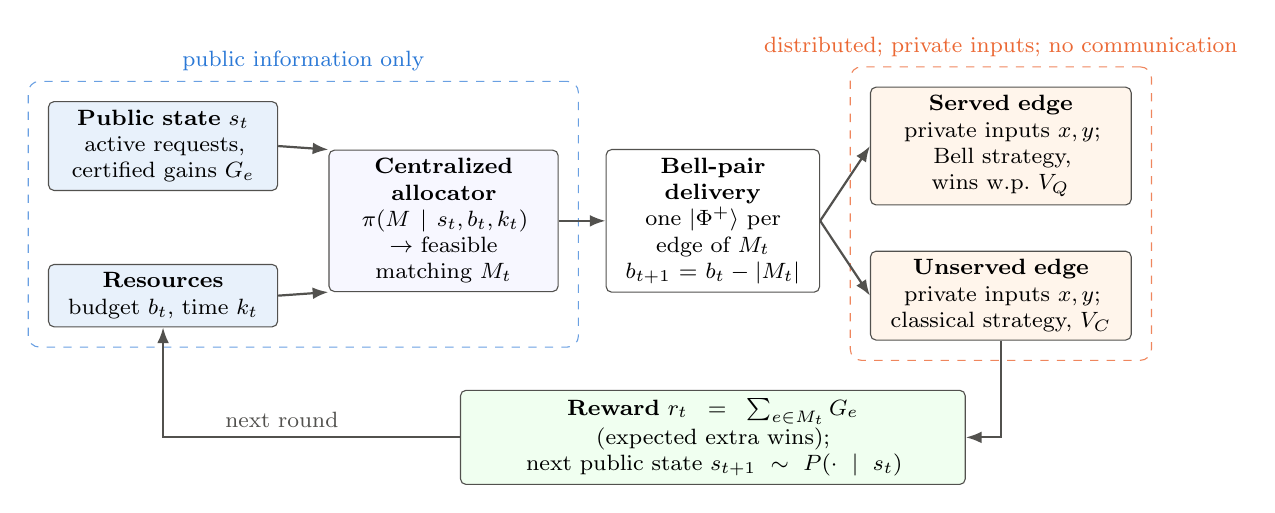
\begin{tikzpicture}[x=0.95cm,
  font=\footnotesize,
  box/.style={draw=inkgray,rounded corners=2pt,align=center,fill=white,inner sep=3pt},
  arr/.style={-{Latex[length=2mm]},thick,inkgray}]
\node[box,fill=softblue,text width=27mm] (state) at (0,0.95) {\textbf{Public state} $s_t$\\active requests,\\certified gains $G_e$};
\node[box,fill=softblue,text width=27mm] (res) at (0,-0.95) {\textbf{Resources}\\budget $b_t$, time $k_t$};
\node[box,fill=blue!3,text width=27mm] (alloc) at (3.75,0) {\textbf{Centralized allocator}\\$\pi(M\mid s_t,b_t,k_t)$\\$\to$ feasible matching $M_t$};
\node[box,text width=25mm] (dist) at (7.35,0) {\textbf{Bell-pair delivery}\\one $|\Phi^+\rangle$ per edge of $M_t$\\$b_{t+1}=b_t-|M_t|$};
\node[box,fill=orange!8,text width=31mm] (q) at (11.2,0.95) {\textbf{Served edge}\\private inputs $x,y$;\\Bell strategy, wins w.p.\ $V_Q$};
\node[box,fill=orange!8,text width=31mm] (c) at (11.2,-0.95) {\textbf{Unserved edge}\\private inputs $x,y$;\\classical strategy, $V_C$};
\node[box,fill=green!6,text width=62mm] (rew) at (7.35,-2.75) {\textbf{Reward} $r_t=\sum_{e\in M_t}G_e$ (expected extra wins);\\next public state $s_{t+1}\sim P(\cdot\mid s_t)$};
\draw[arr] (state.east) -- (alloc.north west);
\draw[arr] (res.east) -- (alloc.south west);
\draw[arr] (alloc) -- (dist);
\draw[arr] (dist.east) -- (q.west);
\draw[arr] (dist.east) -- (c.west);
\draw[arr] (c.south) |- (rew.east);
\draw[arr] (rew.west) -| node[pos=0.3,above]{next round} (res.south);
\begin{scope}[on background layer]
\node[draw=ppoblue!70,dashed,rounded corners,fit=(state)(res)(alloc),inner sep=2.5mm] (pubbox) {};
\node[draw=dqnorange!80,dashed,rounded corners,fit=(q)(c),inner sep=2.5mm] (privbox) {};
\end{scope}
\node[anchor=south,text=ppoblue] at (pubbox.north) {public information only};
\node[anchor=south,text=dqnorange] at (privbox.north) {distributed; private inputs; no communication};
\end{tikzpicture}
\caption{One round of budgeted entanglement routing. The allocator is centralized and uses public information only. The endpoint games are distributed and use private inputs. Each served edge consumes one Bell pair, and unused pairs carry over to later rounds.}
\label{fig:overview}
\end{figure}

\begin{figure}[t]
\centering
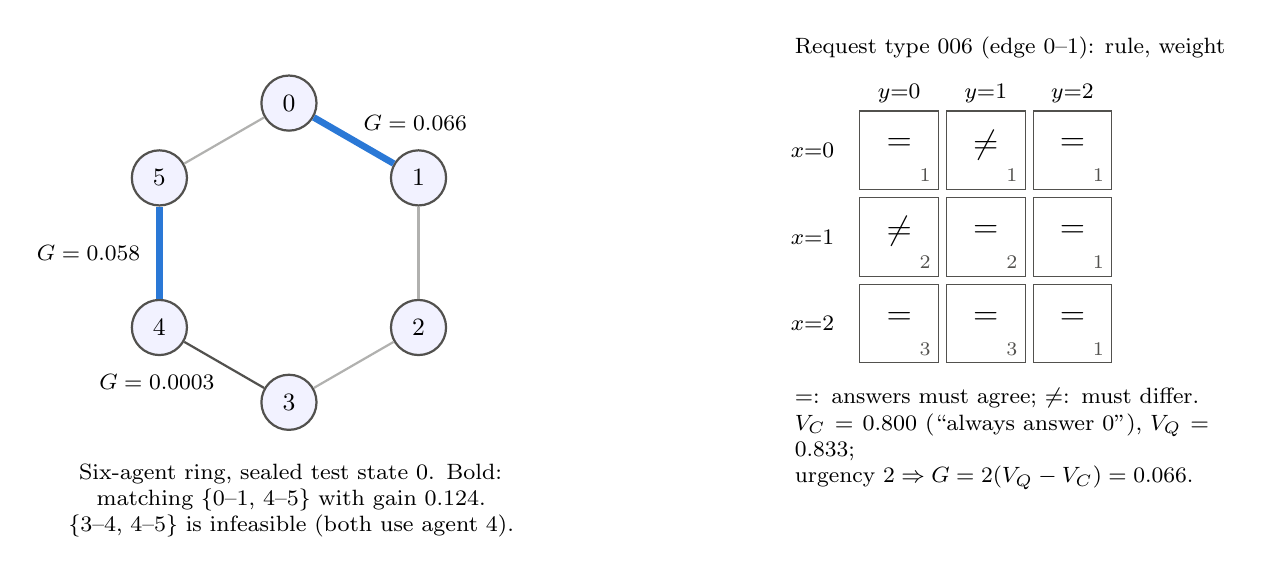
\begin{tikzpicture}[font=\small,
  ag/.style={circle,draw=inkgray,thick,minimum size=7mm,fill=blue!5,inner sep=0pt},
  idle/.style={inkgray!45,thick},
  req/.style={thick,inkgray}]
\begin{scope}
\foreach \i/\ang in {0/90,1/30,2/-30,3/-90,4/-150,5/150} {\node[ag] (a\i) at (\ang:1.9) {\i};}
\draw[idle] (a1)--(a2); \draw[idle] (a2)--(a3); \draw[idle] (a5)--(a0);
\draw[ppoblue,line width=2.4pt] (a0)--(a1);
\draw[req] (a3)--(a4);
\draw[ppoblue,line width=2.4pt] (a4)--(a5);
\node[font=\footnotesize,anchor=south west] at ($(a0)!0.5!(a1)$) {$G=0.066$};
\node[font=\footnotesize,anchor=north east] at ($(a3)!0.5!(a4)$) {$G=0.0003$};
\node[font=\footnotesize,anchor=east] at ($(a4)!0.5!(a5)+(-0.12,0)$) {$G=0.058$};
\node[align=center,font=\footnotesize,text width=62mm] at (0,-3.15) {Six-agent ring, sealed test state 0. Bold: matching $\{0\text{--}1,\,4\text{--}5\}$ with gain $0.124$. $\{3\text{--}4,\,4\text{--}5\}$ is infeasible (both use agent 4).};
\end{scope}
\begin{scope}[xshift=7.2cm,yshift=1.3cm]
\node[font=\footnotesize,anchor=west] at (-0.9,1.3) {Request type 006 (edge 0--1): rule, weight};
\foreach \k in {0,1,2} {\node[font=\footnotesize] at (-0.55,-1.1*\k) {$x{=}\k$}; \node[font=\footnotesize] at (0.55+1.1*\k,0.72) {$y{=}\k$};}
\foreach \x/\y/\r/\w in {0/0/=/1,0/1/\neq/1,0/2/=/1,1/0/\neq/2,1/1/=/2,1/2/=/1,2/0/=/3,2/1/=/3,2/2/=/1} {
  \pgfmathsetmacro{\cx}{0.55+1.1*\y}\pgfmathsetmacro{\cy}{-1.1*\x}
  \node[draw=inkgray,minimum size=10mm,fill=white] at (\cx,\cy) {};
  \node at (\cx,\cy+0.07) {\large$\r$};
  \node[font=\scriptsize,text=inkgray] at (\cx+0.33,\cy-0.32) {\w};}
\node[align=left,font=\footnotesize,anchor=north west,text width=55mm] at (-0.9,-2.9) {$=$: answers must agree; $\neq$: must differ.\\$V_C=0.800$ (``always answer 0''), $V_Q=0.833$;\\urgency $2\Rightarrow G=2(V_Q-V_C)=0.066$.};
\end{scope}
\end{tikzpicture}
\caption{A public request graph and one request. \emph{Left:} gains $G_e$ of the three active requests in the first state of the sealed six-agent ring. Spending a pair on edge $3$--$4$ would waste it. \emph{Right:} the winning rule of the request on edge $0$--$1$. The small numbers are the integer input weights $w_{xy}$.}
\label{fig:example}
\end{figure}

\subsection{Resource-noise models}\label{sec:noise-model}

We consider two independent imperfections of the delivered pairs.
\begin{itemize}[leftmargin=*]
  \item \textbf{Werner noise.} The delivered state is $\rho_v=v\,|\Phi^+\rangle\langle\Phi^+|+(1-v)\,I/4$ \cite{werner1989quantum}. All correlations $\E[(-1)^{a\xor b}]$ scale by $v$, so the Bell value becomes $V_Q^{(v)}=\tfrac12+v\,(V_Q-\tfrac12)$, and the gain is $u_e\max\{0,V_Q^{(v)}-V_C\}$. A request keeps a positive gain only if $v>v^*(\tau)=(V_C-\tfrac12)/(V_Q-\tfrac12)$. Its endpoints fall back to the classical strategy otherwise, so the surplus can reach zero but never goes negative. The allocator observes these noisy gains.
  \item \textbf{Heralded generation loss.} Each attempted pair independently succeeds with probability $p_h$ and is consumed either way. A failed edge falls back to the classical strategy. Allocators observe the ideal gains and are not told $p_h$.
\end{itemize}

%======================================================================
\section{Allocators and reference methods}\label{sec:methods}
%======================================================================

All allocators act on the same public state, the same feasible set (\cref{eq:feasible}), and the same paired evaluation sequences. They differ in what additional information they use and in whether they learn. \Cref{tab:fairness} summarises the differences.

\subsection{Shared observation and encoder for the learned allocators}\label{sec:features}

All four learned methods use a graph-size-independent, permutation-invariant encoding \cite{zaheer2017deep} that supports up to eight agents (28 edge slots). For a candidate action $M$, each edge slot $e$ carries the triple $(10\,G_e,\ \mathbf{1}[e\in E_{s}],\ \mathbf{1}[e\in M])$. Eight global features are appended: remaining budget $b/B$, remaining time $k/H$, agent count $n/8$, $|M|/2$, $10\,G(M)$, $10\max_{e}G_e$, $10\,\mathrm{mean}_{e\in E_s}G_e$, and $|E_s|/28$. A shared two-layer ReLU edge network (width 64) is mean-pooled over the active edges, concatenated with the global features, and passed to a two-layer head that outputs a scalar score for $(s,b,k,M)$. Scoring each feasible joint action in this way enforces the matching and budget constraints by construction, since infeasible actions are never scored. None of the learners observes the transition matrix, the private inputs, or future states.

\subsection{Learned allocators}\label{sec:learners}

\paragraph{DQN.} The score network is an action-value function $Q_\theta(s,b,k,M)$ \cite{mnih2015human}. Transitions are stored in a replay buffer of 20{,}000 entries. With minibatches of 64 and the Huber loss, the undiscounted finite-horizon target is
\begin{equation}
  y = 10\,r_t + \mathbf{1}[t<H]\max_{M'\in\M(s_{t+1},b_{t+1})} Q_{\bar\theta}(s_{t+1},b_{t+1},k_t-1,M'),
\end{equation}
with target parameters $\bar\theta$ copied every 200 updates. Exploration is $\varepsilon$-greedy, with $\varepsilon$ decaying linearly from 1 to 0.03 over the first 65\% of episodes. Evaluation acts greedily on $Q_\theta$.

\paragraph{Double DQN.} Identical to DQN, except that the online network selects and the target network evaluates the next action \cite{vanhasselt2016deep}: $y=10\,r_t+Q_{\bar\theta}\bigl(s',b',k',\arg\max_{M'}Q_\theta(s',b',k',M')\bigr)$.

\paragraph{PPO.} The score network outputs logits of a categorical policy $\pi_\theta(M\mid s,b,k)$ over the feasible matchings. A second encoder of the same architecture provides a state value $V_\phi$ \cite{schulman2017proximal}. Rollouts of 16 episodes are followed by 4 full-batch epochs of the clipped surrogate objective (clip 0.2), a value loss (coefficient 0.5), and an entropy bonus (0.01), using undiscounted Monte Carlo returns. Implementation detail retained as frozen: the value head is regressed on standardized returns, while the advantage subtracts its raw output from unstandardized returns. It therefore acts as a learned state-dependent offset rather than a calibrated baseline. Evaluation takes the most probable matching.

\paragraph{Recurrent PPO.} As PPO, except that a GRU cell \cite{cho2014learning} (width 64) integrates the pooled state encoding and global features across rounds. Each candidate matching is scored from the hidden state and two action features, $|M|/2$ and $10\,G(M)$. The hidden state is reset at episode start.

All learners use Adam \cite{kingma2015adam} with gradient-norm clipping at 5 and scale rewards by 10 during training. The configuration selected for every method in development was width 64 and learning rate $10^{-3}$ (\cref{sec:development}). DQN and Double DQN have \paramsDQN{} parameters. PPO has \paramsPPO{} parameters (policy plus value network).

\subsection{Non-learned allocators}\label{sec:baselines}

\paragraph{Classical exact.} Uses no Bell pairs. Every request is answered with its optimal deterministic classical strategy (\cref{eq:classical}). Its surplus is zero by definition, and it anchors the surplus scale.

\paragraph{Random.} Samples uniformly from $\M(s_t,b_t)$, including the empty matching. It uses neither gains nor future information and tests whether arbitrary use of the budget is sufficient.

\paragraph{Static.} Assigns each edge slot a fixed priority equal to its mean certified gain over the development and validation catalogs, then picks the feasible matching with the largest total priority (breaking ties towards more pairs). It never adapts to the current gains. Because edge indices do not correspond to the same agent pairs across topologies, the priorities are a crude index-level prior. This control tests whether a fixed deployment plan can replace state-dependent allocation.

\paragraph{Greedy (myopic).} Picks $\arg\max_{M\in\M(s_t,b_t)}G(M)$ with $G(M)=\sum_{e\in M}G_e$, breaking ties towards more pairs. It sees the current gains and budget but ignores the remaining time and the future, so it spends whenever any positive gain is visible. It is the primary non-learned comparator.

\subsection{Reference solutions (not equal-information competitors)}\label{sec:references}

\paragraph{Online model-aware dynamic programming (online DP).} Knows the true transition matrix $P$ and solves the finite-horizon Bellman recursion exactly,
\begin{equation}
  W_k(s,b)=\max_{M\in\M(s,b)}\Bigl[G(M)+\sum_{s'}P(s'\mid s)\,W_{k-1}(s',b-|M|)\Bigr],\qquad W_0\equiv0,
\end{equation}
and acts on it. It is the optimal non-anticipative policy in expectation for the ideal-resource objective \cite{puterman1994markov}, so it measures the headroom available to any allocator without future knowledge.

\paragraph{Future-clairvoyant.} Knows the realized future state sequence and solves the same recursion along it. It is an unattainable ceiling that quantifies the value of foresight.

\paragraph{Message oracle.} Lets the endpoints exchange their private inputs, so every request can be won with certainty without any Bell pair, budget, or matching constraint. Its value $\sum_t\sum_{e\in E_{s_t}}u_e(1-V_C)$ is on a different scale and serves only as a reminder that communication, when available, dominates entanglement. It is excluded from all fairness claims.

\begin{table}[t]
\centering
\caption{Fairness and role of every allocator. ``Gains'' are the certified public gains $G_e$ of the current state. No method observes the endpoints' private inputs. The learned methods share one observation contract, training split, episode budget, tuning budget (three configurations, two seeds each), and checkpoint rule.}
\label{tab:fairness}
\footnotesize
\setlength{\tabcolsep}{4pt}
\begin{tabularx}{\textwidth}{@{}l>{\raggedright\arraybackslash}Xc>{\raggedright\arraybackslash}p{27mm}>{\raggedright\arraybackslash}p{40mm}@{}}
\toprule
Method & Observes & Bell budget & Model / future access & Role \\
\midrule
Classical exact & nothing (fixed optimal classical strategies) & 0 & none & defines zero surplus \\
Random & feasible set only & $B$ & none & control: indiscriminate spending \\
Static & feasible set; fixed edge priorities & $B$ & non-test gain averages & control: fixed deployment plan \\
Greedy & current gains; budget & $B$ & none & myopic comparator \\
DQN & gains, active edges, $b/B$, $k/H$, $n$ & $B$ & none (learned) & learned comparator \\
Double DQN & as DQN & $B$ & none (learned) & development candidate \\
PPO & as DQN & $B$ & none (learned) & locked primary method \\
Recurrent PPO & as DQN, plus GRU memory & $B$ & none (learned) & development candidate \\
Online DP & state, budget, time & $B$ & true transition matrix & model-aware headroom reference \\
Future-clairvoyant & entire realized sequence & $B$ & realized future & unattainable ceiling \\
Message oracle & private inputs (communication) & n/a & communication & different resource; excluded \\
\bottomrule
\end{tabularx}
\end{table}

%======================================================================
\section{Experimental protocol}\label{sec:protocol}
%======================================================================

\subsection{Staged preregistration}\label{sec:stages}

The study ran as a sequence of stages, each on its own permanent version-control branch. Each stage committed and published its source, configuration, and hash-locked inputs before any reportable execution. Its raw records, diagnostics, and checkpoints were archived as hash-inventoried bundles. An earlier locked four-agent study (\emph{Study~I}, \cref{sec:studyone}) motivated the extension. The extension then proceeded as follows. Stage~25 generated fresh request types and catalogs and hash-locked the test split. Stage~26 tuned the four learners and ran input ablations on non-test data. Stage~27 measured robustness and scaling on validation catalogs and froze the confirmatory design. Stage~28 opened the sealed test split exactly once. Stage~29 independently re-derived every reported number from raw rows (\cref{sec:audit}).

\subsection{Data splits}\label{sec:splits}

Request types were generated independently per split: 18 development, 12 validation, and 16 test types, with disjoint identifiers and disjoint (predicate, weight) contents. \Cref{tab:catalogs} lists the catalogs. Stage-28 learners trained on all 12 development and validation catalogs (three to six agents) and were evaluated on the four sealed test catalogs. These were designed to probe fresh requests on a four-agent complete graph, an unseen six-agent ring, an unseen eight-agent sparse graph with budget 10, and a horizon-24 path.

\paragraph{Disclosed overlap of public dynamics.} The independent audit (\cref{sec:audit}) found that the catalog generator derived each catalog seed as (split seed) $+\,100\,+$ (catalog offset), which made seeds collide across splits. As a result, two sealed test catalogs reuse the \emph{public dynamics} of training catalogs: the transition matrix, the active-edge-index pattern, and the urgencies. Their \emph{request types} are fresh. The four-agent complete test catalog has the same dynamics as the development four-agent complete catalog. The horizon-24 path shares its state process with the development four-agent star, but has a different graph, matching structure, horizon, and budget. One validation catalog (three-agent ring) likewise duplicates a development catalog. The six-agent ring and eight-agent sparse test catalogs are fully fresh. The registered analysis is unchanged and reported as locked. We add a clearly labelled post hoc sensitivity analysis restricted to the two fully fresh catalogs (\cref{sec:transfer}).

\begin{table}[t]
\centering
\caption{Catalogs. Every catalog has 14 public states and at most two simultaneous pairs per round. $n$: agents; $|E|$: public edges; $H$: horizon; $B$: Bell-pair budget.}
\label{tab:catalogs}
\small
\begin{tabularx}{\textwidth}{@{}l>{\raggedright\arraybackslash}Xccccc>{\raggedright\arraybackslash}p{30mm}@{}}
\toprule
Split & Topologies & $n$ & $|E|$ & $H$ & $B$ & Use \\
\midrule
Development (8) & path, ring (3 agents); complete, path, ring, star (4); path, star (6) & 3--6 & 2--6 & 8--16 & 2--6 & Stage 26 tuning; Stage 28 training \\
Validation (4) & ring (3); sparse random (4); path, star (6) & 3--6 & 3--5 & 8--16 & 2--6 & Stages 26--27 selection; Stage 28 training \\
\midrule
Test & complete (fresh requests$^\dagger$) & 4 & 6 & 10 & 6 & sealed; Stage 28 only \\
Test & ring (unseen size) & 6 & 6 & 16 & 6 & sealed; fully fresh \\
Test & sparse random (unseen size) & 8 & 11 & 24 & 10 & sealed; fully fresh \\
Test & path (long horizon$^\dagger$) & 4 & 3 & 24 & 6 & sealed; Stage 28 only \\
\bottomrule
\end{tabularx}\\[2pt]
{\footnotesize $^\dagger$Public dynamics shared with a development catalog (see text); request types are fresh.}
\end{table}

\subsection{Training protocol}\label{sec:training}

In development (Stage~26) each learner received three configurations of (width, learning rate): $(32,3{\times}10^{-4})$, $(64,3{\times}10^{-4})$, and $(64,10^{-3})$ for DQN and Double DQN, and $(32,10^{-4})$, $(64,3{\times}10^{-4})$, and $(64,10^{-3})$ for PPO and recurrent PPO. Each configuration had two seeds, 1{,}200 training episodes per seed, and 300 paired validation sequences per catalog. Selection used the final checkpoint only. In the locked study (Stage~28), 12 fresh DQN and 12 fresh PPO models (seeds 28000--28011) were each trained for 2{,}500 episodes, cycling through the 12 training catalogs. Training used ideal resources and expected rewards. Only the final checkpoint of each model was evaluated, without any selection.

\subsection{Locked confirmatory design}\label{sec:design}

Each final checkpoint was evaluated on the same 500 paired sequences per sealed catalog (sequence seeds 228000--228499). The 7 non-learned methods saw the same sequences. The primary unit is the training seed. For seed $i$ and method $m$, let $\bar S^{(m)}_i$ be the mean surplus over sequences, averaged with equal weight over the four catalogs. The three registered primary tests, all reported regardless of outcome, are as follows.
\begin{enumerate}[leftmargin=*]
  \item \textbf{PPO superior to DQN:} the 95\% percentile bootstrap interval of $\overline{\bar S^{\mathrm{PPO}}_i-\bar S^{\mathrm{DQN}}_i}$ has lower bound $>0$.
  \item \textbf{PPO superior to greedy:} the 95\% interval of $\overline{\bar S^{\mathrm{PPO}}_i}-S^{\mathrm{greedy}}$ has lower bound $>0$ (greedy is deterministic).
  \item \textbf{PPO--DQN practical equivalence:} the two-sided 90\% interval of the paired difference lies entirely within $\pm\delta$, with $\delta=0.05\times$ the online-DP mean surplus. This is an interval-inclusion version of two one-sided tests at level 0.05 \cite{schuirmann1987comparison}.
\end{enumerate}
Intervals use 20{,}000 seed-level resamples with fixed seeds \cite{efron1993introduction}. Tests 1 and 3 can both fail or both pass, and both are reported. Secondary per-catalog contrasts (PPO $>$ DQN) use exact one-sided Wilcoxon signed-rank tests over the 12 seed pairs \cite{wilcoxon1945individual} with Holm adjustment across the four catalogs \cite{holm1979simple}. The secondary noisy-resource conditions ($v\in\{0.8,0.6\}$ and $p_h\in\{0.75,0.5\}$) evaluate the 12 PPO models on the first 100 sequences per catalog, fixed in advance to respect the compute cap. The execution gates required all 24 models, every catalog and condition, finite values, and zero budget or matching violations within 4 active wall-hours and 2.5 million allocator decisions. A scientific null result passes the execution gate when it is complete and correctly reported.

%======================================================================
\section{Results}\label{sec:results}
%======================================================================

\subsection{Study I: a fixed four-agent benchmark}\label{sec:studyone}

The first locked study used a single four-agent complete graph (6 edges, $H=10$, $B=6$), 12 sealed request types, a masked DQN allocator (termed BER-MARL there), 16 training seeds, and 1{,}000 paired test sequences. The learned allocator reached mean surplus \sOneBer, compared with \sOneGreedy{} for greedy, \sOneRandom{} for random, \sOneStatic{} for static, \sOneDP{} for online DP, and \sOneFuture{} for the future-clairvoyant ceiling. The paired difference from greedy was \sOneDiff{} (95\% CI [\sOneDiffLo, \sOneDiffHi]), and all \sOneSeedsAbove{} seeds exceeded greedy. The allocator recovered \sOneFrac\% of the online-DP surplus. A preregistered stronger gate required the one-sided 95\% lower bound of this fraction to exceed 90\%. That gate \textbf{failed}, with a lower bound of \sOneFracLo\%. Study~I thus supported a learned-versus-greedy advantage and gave a null result for near-optimality. Its single graph motivated the multi-topology extension below.

\subsection{Development: learners and input ablations}\label{sec:development}

In development the four learners were nearly indistinguishable on validation catalogs: DQN \develDQN, Double DQN \develDDQN, PPO \develPPO, and recurrent PPO \develRPPO{} (\cref{fig:ablation}b). The registered development hypothesis was that Double DQN would beat the strongest other learner. It was \textbf{not supported}: Double DQN minus PPO was \develDDQNMinusPPO. PPO became the locked primary method and DQN its learned comparator.

The input ablations were much larger than the algorithm differences (\cref{fig:ablation}a). Starting from Double DQN with the full public resource state (\develDDQN), removing the remaining-budget input reduced validation surplus to \ablNoBudget{} ($-$\ablDropNoBudget\%). Replacing gain magnitudes by binary indicators gave \ablBinary{} ($-$\ablDropBinary\%). Assigning gains to the wrong active edges gave \ablShuffled{} ($-$\ablDropShuffled\%). Removing the remaining-time input gave \ablNoHorizon{} ($-$\ablDropNoHorizon\%). Learned allocation therefore depends on knowing \emph{how much} each request gains, \emph{where} that gain sits on the graph, \emph{how many} pairs remain, and \emph{how much time} remains to use them. The particular optimizer matters much less. These ablations ran on development data with two seeds each and are mechanistic evidence, not confirmatory tests.

\begin{figure}[t]
\centering
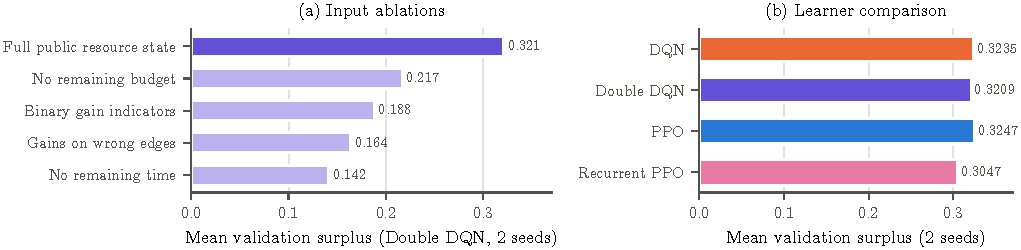
\includegraphics[width=\textwidth]{figures/fig_ablation.pdf}
\caption{Development results on validation catalogs (Stage 26). \emph{(a)} Input ablations of the Double-DQN allocator: removing resource-state or gain information sharply reduces surplus. \emph{(b)} The four independently tuned learners are close to one another, and the preregistered Double-DQN superiority hypothesis was not supported. Source data: \texttt{fig\_ablation\_stage26.csv}, \texttt{fig\_stage26\_methods.csv}.}
\label{fig:ablation}
\end{figure}

\subsection{Locked confirmatory results}\label{sec:confirm}

All 24 models trained and were evaluated without incident. There were no budget, matching, or invalid-action violations, and every execution gate passed. \Cref{tab:main} and \cref{fig:main} report mean surplus by catalog.

\begin{table}[t]
\centering
\caption{Locked evaluation on the sealed catalogs: mean surplus over the classical optimum. Learned rows average 12 seeds $\times$ 500 sequences; baseline rows average the same 500 sequences. ``Overall'' weights the four catalogs equally. Parentheses: percentage of the online-DP surplus on the same catalog.}
\label{tab:main}
\small
\setlength{\tabcolsep}{4.5pt}
\begin{tabular}{@{}lccccc@{}}
\toprule
Method & \shortstack{4-agent\\complete} & \shortstack{6-agent\\ring} & \shortstack{8-agent\\sparse} & \shortstack{4-agent path\\($H{=}24$)} & Overall \\
\midrule
Classical exact & 0 & 0 & 0 & 0 & 0 \\
Random & \catCmpRandom & \catRingRandom & \catSparseRandom & \catPathRandom & \meanRandom \\
Static & \catCmpStatic & \catRingStatic & \catSparseStatic & \catPathStatic & \meanStatic \\
Greedy & \catCmpGreedy{} (\fracCmpGreedy) & \catRingGreedy{} (\fracRingGreedy) & \catSparseGreedy{} (\fracSparseGreedy) & \catPathGreedy{} (\fracPathGreedy) & \meanGreedy{} (\fracGreedy) \\
DQN & \textbf{\catCmpDQN} (\fracCmpDQN) & \catRingDQN{} (\fracRingDQN) & \textbf{\catSparseDQN} (\fracSparseDQN) & \catPathDQN{} (\fracPathDQN) & \textbf{\meanDQN} (\fracDQN) \\
PPO & \catCmpPPO{} (\fracCmpPPO) & \textbf{\catRingPPO} (\fracRingPPO) & \catSparsePPO{} (\fracSparsePPO) & \textbf{\catPathPPO} (\fracPathPPO) & \meanPPO{} (\fracPPO) \\
\midrule
Online DP (model-aware) & \catCmpOnline & \catRingOnline & \catSparseOnline & \catPathOnline & \meanOnline \\
Future-clairvoyant & \catCmpFuture & \catRingFuture & \catSparseFuture & \catPathFuture & \meanFuture \\
Message oracle$^\ast$ & \catCmpMessage & \catRingMessage & \catSparseMessage & \catPathMessage & \meanMessage \\
\bottomrule
\end{tabular}\\[2pt]
{\footnotesize $^\ast$Different resource (free communication, no budget); not comparable.}
\end{table}

\begin{figure}[t]
\centering
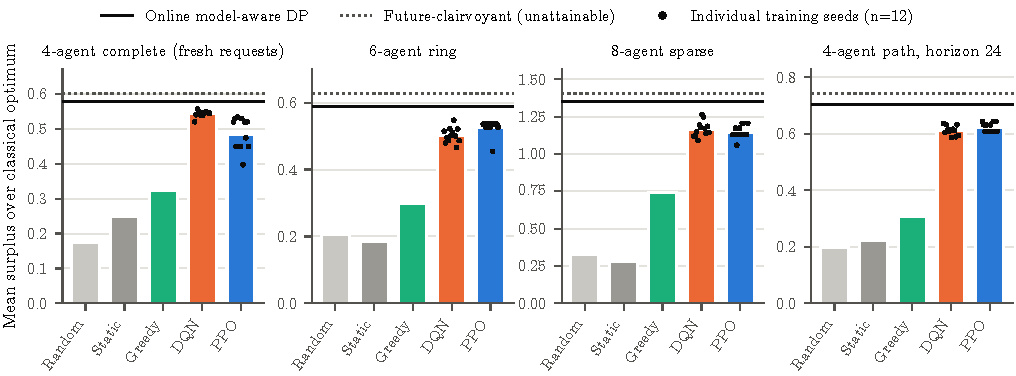
\includegraphics[width=\textwidth]{figures/fig_main_by_catalog.pdf}
\caption{Mean surplus on the four sealed catalogs. Bars give method means; black dots are the 12 individual DQN and PPO training seeds; horizontal lines mark the online model-aware DP reference (solid) and the unattainable future-clairvoyant ceiling (dotted). Source data: \texttt{fig\_main\_by\_catalog.csv}, \texttt{fig\_seed\_catalog.csv}.}
\label{fig:main}
\end{figure}

\paragraph{Primary tests.} The registered outcomes are shown in \cref{fig:intervals} and \cref{tab:tests}.
\begin{enumerate}[leftmargin=*]
  \item \emph{PPO superior to DQN: not supported (null).} The mean paired difference was \ppoMinusDqn, with 95\% CI [\ppoMinusDqnLoNinetyFive, \ppoMinusDqnHiNinetyFive]. PPO exceeded DQN on only \ppoSeedsAboveDqn{} of 12 seeds.
  \item \emph{PPO superior to greedy: supported.} The difference was \ppoMinusGreedy, with 95\% CI [\ppoMinusGreedyLo, \ppoMinusGreedyHi], and all \ppoSeedsAboveGreedy{} PPO seeds exceeded greedy. DQN exceeded greedy by \dqnMinusGreedy, also on all \dqnSeedsAboveGreedy{} seeds.
  \item \emph{PPO--DQN practical equivalence: supported.} The 90\% CI [\ppoMinusDqnLoNinety, \ppoMinusDqnHiNinety] lies inside $\pm\delta=\pm\eqMargin$ (5\% of the online-DP mean \onlineMean).
\end{enumerate}
The 90\% interval excludes zero on the DQN side. No DQN-superiority test was registered, so we read this only as \emph{equivalence within the preregistered margin with a small numerical edge for DQN}, not as evidence that DQN is better. A second, independently seeded bootstrap stream reproduced all three decisions (\cref{sec:audit}).

\begin{figure}[t]
\centering
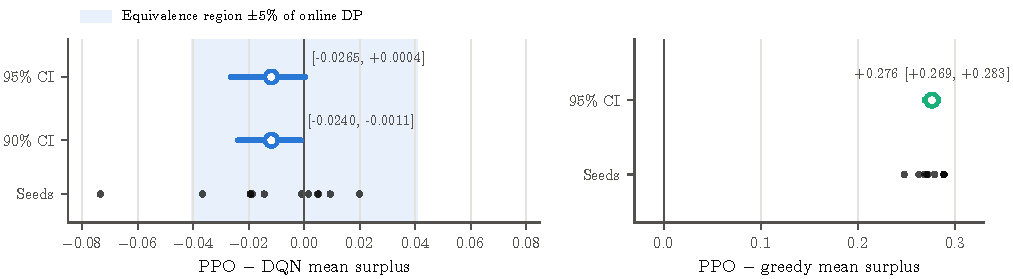
\includegraphics[width=\textwidth]{figures/fig_primary_intervals.pdf}
\caption{Registered primary contrasts with seed-level percentile bootstrap intervals (20{,}000 resamples). \emph{Left:} PPO minus DQN. The 95\% interval used for the superiority test crosses zero (null), while the 90\% interval used for the equivalence test lies inside the shaded $\pm5\%$-of-online-DP region (equivalent). \emph{Right:} PPO minus greedy (superior). Dots are individual seeds. Source data: \texttt{fig\_primary\_intervals.csv}, \texttt{fig\_seed\_contrasts.csv}.}
\label{fig:intervals}
\end{figure}

\begin{table}[t]
\centering
\caption{Registered tests. Primary: seed-level percentile bootstrap intervals. Secondary: exact one-sided Wilcoxon signed-rank tests (PPO $>$ DQN, 12 seed pairs) with Holm adjustment over four catalogs.}
\label{tab:tests}
\small
\begin{tabular}{@{}lrrl@{}}
\toprule
Primary contrast & Estimate & Interval & Decision \\
\midrule
PPO $-$ DQN (superiority) & \ppoMinusDqn & 95\%: [\ppoMinusDqnLoNinetyFive, \ppoMinusDqnHiNinetyFive] & not supported \\
PPO $-$ DQN (equivalence, $\pm\eqMargin$) & \ppoMinusDqn & 90\%: [\ppoMinusDqnLoNinety, \ppoMinusDqnHiNinety] & supported \\
PPO $-$ greedy (superiority) & \ppoMinusGreedy & 95\%: [\ppoMinusGreedyLo, \ppoMinusGreedyHi] & supported \\
\midrule
Secondary catalog & PPO $-$ DQN & PPO seed wins & raw $p$ / Holm $p$ \\
\midrule
4-agent complete & \diffCmp & \winsCmp/12 & \rawpCmp{} / \holmpCmp \\
6-agent ring & \diffRing & \winsRing/12 & \rawpRing{} / \holmpRing \\
8-agent sparse & \diffSparse & \winsSparse/12 & \rawpSparse{} / \holmpSparse \\
4-agent path, $H=24$ & \diffPath & \winsPath/12 & \rawpPath{} / \holmpPath \\
\bottomrule
\end{tabular}
\end{table}

\paragraph{Secondary catalog contrasts.} No per-catalog PPO advantage survives Holm adjustment at $\alpha=0.05$ (\cref{tab:tests}). The direction varies by catalog. PPO is ahead on the ring (\winsRing/12 seeds) and the long path, and behind on the complete graph (\winsCmp/12) and the sparse eight-agent graph. These sign changes are consistent with two equivalent learners that make slightly different trade-offs on each graph. The largest DQN lead, on the four-agent complete catalog (\fracCmpDQN\% of online DP), occurs on the test catalog whose public dynamics coincide with a training catalog. We do not interpret it causally.

\paragraph{How far from the model-aware optimum?} Overall, the learned allocators recovered \fracPPO\% (PPO) and \fracDQN\% (DQN) of the online-DP surplus, compared with \fracGreedy\% for greedy. The unattainable future-clairvoyant ceiling lies only slightly above online DP (\fracFuture\% of it). The learners' remaining gap to online DP is therefore about three times larger than the value of perfect foresight. Better model-free credit assignment, or partial model knowledge, therefore has more to offer than prediction of the future. The PPO seeds also collapsed onto only \ppoDistinctSeedValues{} distinct seed-level outcomes out of 12. Several seeds converged to identical deterministic (argmax) allocation rules. The seed bootstrap remains valid for the distribution of training outcomes, but PPO's effective policy diversity is lower than its seed count.

\subsection{Transfer across topology, size, and horizon}\label{sec:transfer}

\Cref{fig:scaling} places the sealed test catalogs beside the Stage-27 validation catalogs as a fraction of online-DP surplus. On the two fully fresh catalogs, the six-agent ring and the eight-agent sparse graph with an unseen size, unseen edge count, and a budget of 10, both learners kept roughly 85--89\% of the model-aware optimum. Greedy kept about 51--55\%. No method was trained on more than six agents. The permutation-invariant encoding transferred to eight agents and 11 edges without retraining.

Because two sealed catalogs share public dynamics with training catalogs (\cref{sec:splits}), we repeated the primary contrasts on the two fully fresh catalogs only. This analysis is post hoc and descriptive, with no decision rule. PPO minus greedy was \phPPOMinusGreedy{} (95\% CI [\phPPOMinusGreedyLo, \phPPOMinusGreedyHi]). PPO minus DQN was \phPPOMinusDqn, with a 90\% CI [\phPPOMinusDqnLoNinety, \phPPOMinusDqnHiNinety] inside the corresponding $\pm5\%$ margin of $\pm\phMargin$. PPO and DQN recovered \phFracPPO\% and \phFracDQN\% of online DP, and greedy \phFracGreedy\%. The qualitative conclusions, a large learned advantage over greedy and practical equivalence of the two learners, do not depend on the overlapping catalogs.

\begin{figure}[t]
\centering
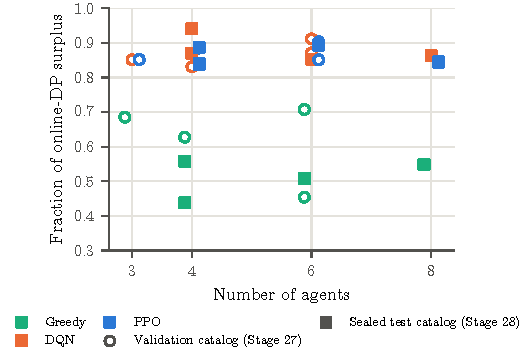
\includegraphics[width=0.62\textwidth]{figures/fig_scaling.pdf}
\caption{Fraction of the online model-aware DP surplus achieved on validation catalogs (Stage 27; open circles; three seeds) and sealed test catalogs (Stage 28; filled squares; 12 seeds), by number of agents. Points are horizontally offset by method. Source data: \texttt{fig\_scaling.csv}.}
\label{fig:scaling}
\end{figure}

\subsection{Noisy resources and the fidelity threshold}\label{sec:noise}

\Cref{tab:noise} and \cref{fig:noise} combine the Stage-27 validation conditions (all four learners, three seeds each, 200 sequences per catalog and condition) with the Stage-28 sealed-test conditions (12 PPO models, 100 sequences per catalog).

\begin{table}[t]
\centering
\caption{Mean surplus under resource imperfections. Validation: Stage 27, three seeds per learner, four validation catalogs. Sealed test: Stage 28, 12 PPO models, the first 100 sequences of each sealed catalog (ideal value on the same 100 sequences).}
\label{tab:noise}
\small
\begin{tabular}{@{}lcccccccc@{}}
\toprule
& Ideal & $p_h{=}0.9$ & $p_h{=}0.75$ & $p_h{=}0.5$ & $v{=}0.9$ & $v{=}0.8$ & $v{=}0.7$ & $v{=}0.6$ \\
\midrule
DQN (val.) & \validDQNIdeal & \validDQNHerNine & \validDQNHerSevenFive & \validDQNHerFive & \validDQNVisNine & \validDQNVisEight & \validDQNVisSeven & \validDQNVisSix \\
Double DQN (val.) & \validDDQNIdeal & \validDDQNHerNine & \validDDQNHerSevenFive & \validDDQNHerFive & \validDDQNVisNine & \validDDQNVisEight & \validDDQNVisSeven & \validDDQNVisSix \\
PPO (val.) & \validPPOIdeal & \validPPOHerNine & \validPPOHerSevenFive & \validPPOHerFive & \validPPOVisNine & \validPPOVisEight & \validPPOVisSeven & \validPPOVisSix \\
Recurrent PPO (val.) & \validRPPOIdeal & \validRPPOHerNine & \validRPPOHerSevenFive & \validRPPOHerFive & \validRPPOVisNine & \validRPPOVisEight & \validRPPOVisSeven & \validRPPOVisSix \\
\midrule
PPO (sealed test) & \noiseIdealHundred & -- & \noiseHerSevenFive & \noiseHerFive & -- & \noiseVisEight & -- & \noiseVisSix \\
\bottomrule
\end{tabular}
\end{table}

\paragraph{Heralded loss: proportional degradation.} On the sealed catalogs, PPO kept \ratioHerSevenFive{} and \ratioHerFive{} of its ideal surplus at $p_h=0.75$ and $0.5$, which is essentially the proportional scaling $p_h$ expected when every attempted pair fails independently (\cref{fig:noise}a). The allocators were trained without loss and are not told $p_h$. They therefore do not adapt to it, and the result shows absence of collapse rather than learned robustness. An allocator that knew $p_h$ could not do better under our model. Every attempt costs one pair whether or not it heralds, and the expected gain of every action scales by the same factor $p_h$, so the optimal ordering of actions is unchanged.

\paragraph{Werner noise: a sharp threshold.} Surplus vanished for every method at $v\le0.8$, on validation and on the sealed family (\cref{fig:noise}b). This collapse belongs to the \emph{request family}, not to the learners. A request retains a positive gain only above its visibility threshold $v^*(\tau)=(V_C-\tfrac12)/(V_Q-\tfrac12)$. On the sealed family the thresholds had minimum \thrTestMin, median \thrTestMedian, and mean \thrTestMean. On the 30 non-test types they had minimum \thrNonTestMin{} and median \thrNonTestMedian. Of the \testOpportunities{} request entries in the sealed catalogs' state tables, \posOppIdeal\% carry a positive gain under ideal pairs, \posOppNineFive\% at $v=0.95$, \posOppNine\% at $v=0.9$, and \posOppEight\% at $v=0.8$ (\cref{fig:noise}c). On validation, \validPosOppNine\% of opportunities kept a positive gain at $v=0.9$. Below about $v=0.85$, no allocator can create value from these games, because the classical fallback is already optimal. The small gaps between classical and quantum values that make the benchmark interesting (typically a few percent of winning probability) are exactly what makes it fragile to depolarizing noise. High-fidelity entanglement is a precondition of the whole effect, not a secondary detail.

\begin{figure}[t]
\centering
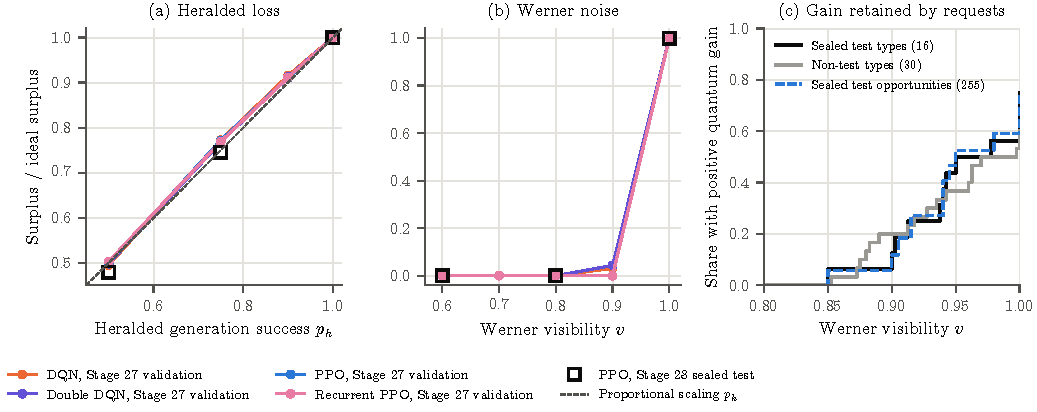
\includegraphics[width=\textwidth]{figures/fig_noise.pdf}
\caption{Resource imperfections. \emph{(a)} Surplus relative to ideal under heralded generation loss closely follows proportional scaling (dashed). \emph{(b)} Under Werner noise the surplus collapses to zero at $v\le0.8$ for every learner. \emph{(c)} Share of request types and of sealed test request occurrences that retain a positive Bell-minus-classical gain at visibility $v$. No sealed request retains a gain at $v=0.8$. Source data: \texttt{fig\_noise\_stage27.csv}, \texttt{fig\_noise\_stage28.csv}, \texttt{fig\_visibility\_thresholds.csv}, \texttt{fig\_positive\_fraction\_test.csv}.}
\label{fig:noise}
\end{figure}

%======================================================================
\section{Independent audit, compute, and quantum-resource accounting}\label{sec:audit}
%======================================================================

\paragraph{Independent reproduction.} A separate audit module re-derived every reported Stage-28 quantity from the 81{,}200 raw episode rows. It does not import the Stage-28 analysis code, the routing environment, or the learners. It reproduced all method means, the three primary intervals, the four exact Wilcoxon $p$-values with their Holm adjustments, the secondary condition means, and the visibility-threshold summary to within $10^{-9}$. It re-checked every sealed request certificate: the exact classical enumeration, the Bell value re-evaluated analytically at the recorded angles, and an independently formulated XOR SDP solved with CVXPY/Clarabel \cite{diamond2016cvxpy}. It verified the SHA-256 of all 24 checkpoints against the archive inventory and loaded each one to confirm method, seed, frozen configuration, episode count, and parameter count. It also checked that every learned episode satisfied attempted $+$ unused $=$ budget. It confirmed that request-type identifiers and contents are disjoint across splits, that the sealed files are byte-identical to their Stage-25 lock commit and were never modified afterwards, that no pre-Stage-28 record mentions a test identifier (other than the hash-locked freeze file), that only one Stage-28 attempt exists, and that only final checkpoints were evaluated. Per-round matchings are not logged. Matching feasibility therefore rests on the evaluator, which raises an error on any infeasible action, and on the empty violation list. The audit also produced the public-dynamics overlap finding of \cref{sec:splits}.

\begin{table}[t]
\centering
\caption{Resource ledger of the locked Stage-28 study. Counters are kept separate. ``Decisions'' are allocator actions. Circuit evaluations are analytic float64 Bell-correlator evaluations during request certification. No shots were sampled and no quantum hardware or GPU was used.}
\label{tab:resources}
\small
\begin{tabular}{@{}lr@{\hspace{10mm}}lr@{}}
\toprule
Counter & Value & Counter & Value \\
\midrule
Training decisions (24 models) & \resTrainDecisions & Allocator optimizer updates & \resAllocUpdates \\
Primary evaluation decisions & \resEvalPrimary & Certification optimizer updates & \resCertUpdates \\
Noisy-condition decisions & \resEvalSecondary & Analytic circuit evaluations & \resCircuits \\
Baseline-policy decisions & \resBaseline & Measurement shots & 0 \\
\textbf{Total decisions} (cap 2{,}500{,}000) & \textbf{\resDecisions} & GPU device-hours & 0 \\
Active wall time (cap 4 h) & \resWallHours{} h & CPU core-hours (1 thread) & \resCPU \\
\bottomrule
\end{tabular}
\end{table}

\paragraph{Compute.} \Cref{tab:resources} lists the Stage-28 ledger. Training took about \resDqnTrain{} s per DQN model and \resPpoTrain{} s per PPO model on one CPU thread. Across the QIP extension (Stages~26--28, including a retained failed bundle and its analysis-only recovery), the experiments used \progDecisions{} allocator decisions, \progUpdates{} optimizer updates, and \progWallHours{} active wall-hours (\progCPU{} CPU core-hours). The independent audit used no allocator decisions and solved 16 small SDPs.

%======================================================================
\section{Discussion}\label{sec:discussion}
%======================================================================

\paragraph{What the evidence supports.} Across two locked studies, model-free allocators trained only on public information learned \emph{when and where} to spend certified Bell pairs. They raised the share of the model-aware optimum achieved from about one half (greedy) to \fracPPO--\fracDQN\%, and they transferred to an eight-agent graph larger than any seen in training. The mechanism ablations and the near-identical performance of four different learners point to the same explanation. The benefit comes from representing the \emph{resource state}, meaning the remaining budget, the remaining time, and the magnitude and location of current gains, not from any one optimization algorithm. The strongest defensible framing is therefore \emph{algorithm-agnostic resource-aware allocation}. Given the right state, standard value-based and policy-gradient learners both close most of the gap between myopic spending and model-aware planning.

\paragraph{What it does not support.} PPO is not superior to DQN; the confirmatory test says the two are practically equivalent within a preregistered margin. Double DQN was not superior in development. Neither study approached the online optimum closely enough to pass the 90\% gate of Study~I. Most importantly, the value of the entire exercise depends on the certified quantum--classical gap. That gap is small for these games and disappears under moderate depolarizing noise.

\paragraph{Why the fidelity threshold matters for quantum networks.} For an application that consumes entanglement through nonlocal correlations, the operational figure of merit is not the entanglement rate alone but the fraction of delivered pairs whose fidelity clears the application's threshold $v^*(\tau)$. In our sealed family, the share of request entries with a positive gain falls from \posOppIdeal\% with ideal pairs to \posOppNineFive\% at $v=0.95$ and \posOppNine\% at $v=0.9$, and reaches zero by $v=0.8$. A routing layer that is unaware of fidelity would spend pairs on requests that its delivered states cannot help. Fidelity-aware gains, as used by our allocators, at least avoid that waste. Purification, or games with larger quantum gaps such as pseudo-telepathy games \cite{brassard2005quantum}, would be needed to make lower-fidelity pairs useful.

%======================================================================
\section{Limitations}\label{sec:limitations}
%======================================================================

\begin{itemize}[leftmargin=*]
  \item \textbf{Request family.} All requests are three-input binary-output XOR games with small certified gaps. Other game families, larger alphabets, or applications with continuous utility could change the allocation problem.
  \item \textbf{Single-hop, centralized model.} Bell pairs are delivered directly between neighbours by a central dispatcher with full public information. Multi-hop swapping, purification, memory decoherence over rounds, and decentralized or partially observed allocation are not modelled.
  \item \textbf{Simulated, expected rewards.} Rewards are analytic expectations over private inputs. No game round is sampled, no quantum circuit is executed during allocation, and there is no hardware experiment.
  \item \textbf{Noise models.} Werner noise and independent heralding are idealized. Learners were trained only on ideal resources, and heralded loss was not observed by the allocator.
  \item \textbf{Split overlap.} Two of four sealed catalogs share public dynamics with training catalogs, as disclosed in \cref{sec:splits}. Transfer claims rest primarily on the six-agent ring and eight-agent sparse catalogs.
  \item \textbf{Scale of the study.} There are 12 seeds per learner, four test catalogs, at most eight agents, and a 14-state public Markov chain per catalog. The tuning grid was small (three configurations), and the selected configuration sat at the edge of the grid (the largest learning rate tested).
  \item \textbf{Implementation details.} The PPO value head is not calibrated to the advantage scale (\cref{sec:learners}). The static baseline uses index-level priorities. Stages~26--28 ran with \texttt{torch 2.15.0} and \texttt{numpy 2.5.4} rather than the versions pinned in the lock file. The actual versions are recorded in every manifest.
  \item \textbf{Novelty.} We are not aware of prior work combining consumable Bell-pair budgets, matching constraints, certified nonlocal-game values, and learned long-horizon allocation. We did not perform a systematic literature review, and readers should treat this positioning as provisional.
\end{itemize}

%======================================================================
\section{Conclusion}\label{sec:conclusion}
%======================================================================

We introduced a benchmark in which a centralized public-information allocator routes scarce, consumable Bell pairs to certified nonlocal-game requests on dynamic graphs. Under a staged, preregistered protocol, learned allocators beat myopic greedy spending by a large and precisely estimated margin and transferred to an unseen eight-agent graph. PPO and DQN were practically equivalent, and neither reached the preregistered near-optimality bar. Resource-state ablations identify budget, time, and gain magnitude and location as the drivers of the effect. The effect is bounded by fidelity: it degrades proportionally under heralded loss and disappears below a Werner visibility of about $0.85$ for this request family. We hope the benchmark, its locked test split, and its complete raw records serve as a reproducible testbed for fidelity-aware entanglement allocation.

%======================================================================
\section*{Statements and declarations}
%======================================================================

\paragraph{Reproducibility.} Every number in this paper is produced by \texttt{docs/paper/make\_numbers.py} from the Stage-29 audit bundle, and every data figure by \texttt{docs/paper/make\_figures.py} from committed CSV source files (\texttt{docs/paper/figure\_data/}). Their SHA-256 hashes are recorded in the audit's \texttt{paper\_tables.json}. Build instructions are in \texttt{docs/paper/BUILD.md}. Each experiment bundle contains its resolved configuration, source commit, runtime manifest, raw append-only metrics, raw episode rows, diagnostics, checkpoints, and a hash inventory, and can be verified with \texttt{python -m eqmarl\_slam.cli verify --run <bundle>}.

\paragraph{Data and code availability.} Source code, configurations, hash-locked data splits, raw experiment records, checkpoints, diagnostics, the audit bundle, figures, and the \LaTeX{} source are publicly available at \url{https://github.com/Youngei402tw/eQMARL-SLAM-Codex}. Each stage has a preserved branch: \texttt{stage/28-qip-confirmatory} for the locked evaluation and \texttt{stage/29-qip-release} for the audit and manuscript. Failed and null runs are retained.

\paragraph{Use of AI tools.} The experiment code, analysis, audit, and drafts of this manuscript were produced with AI coding assistants (OpenAI Codex and Anthropic Claude) operating under the author's direction within a recorded, version-controlled protocol. The author reviewed the work and takes responsibility for its content.

\paragraph{Funding.} No specific funding was received for this work.

\paragraph{Competing interests.} The author declares no competing interests.

\paragraph{Author contributions.} Y.-C.~L.\ conceived the study, directed its design and execution, and wrote and approved the manuscript.

\small
\bibliographystyle{unsrtnat}
\bibliography{QIP_ROBUST_ENTANGLEMENT_ROUTING}

\end{document}
